% !TeX program = pdflatex
\documentclass[tikz,border=8pt]{standalone}
\usepackage{tikz}
\definecolor{FigureBlue}{HTML}{2563EB}\definecolor{FigureOrange}{HTML}{EA580C}
\begin{document}
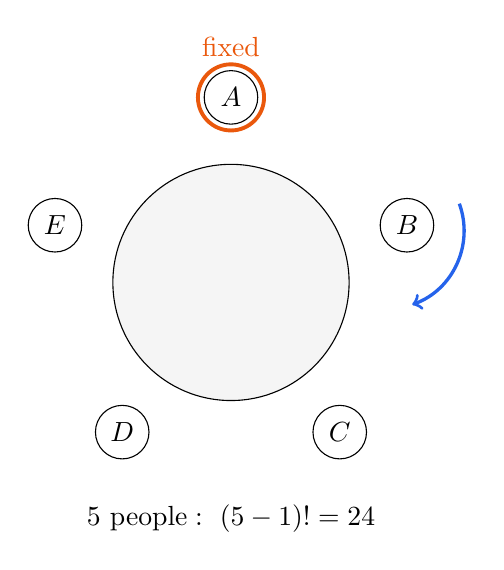
\begin{tikzpicture}
  \draw[fill=gray!8] (0,0) circle (1.5);
  \foreach \ang/\lab in {90/A,18/B,306/C,234/D,162/E}{\coordinate (\lab) at (\ang:2.35);\draw[fill=white] (\lab) circle (.34);\node at (\lab) {$\lab$};}
  \draw[FigureOrange,line width=1.4pt] (A) circle (.42); \node[FigureOrange,above=4mm] at (A) {fixed};
  \draw[->,FigureBlue,line width=1.2pt] (2.9,1) arc[start angle=20,end angle=-70,radius=1];
  \node at (0,-3) {$5\ \mathrm{people}:\ (5-1)!=24$};
\end{tikzpicture}
\end{document}
